\section{Extension to non-Holonomic Constraints}%
\label{sec:non_holonomic_constraints}
%
Mobile manipulators are often equipped with a non\hyp{}holonomic base (e.g., a
differential drive mobile robot). In contrast to revolute joints for
manipulators, non\hyp{}holonomic bases imply non\hyp{}holonomic constraints. Based on
ideas presented in \cite{Meng2019}, we propose a method to integrate such
constraints in optimization fabrics, including \ac{df}.

We assume that the non\hyp{}holonomic constraint at hand can be expressed as an
equality of form
\begin{equation}
  \xdot = \Jnh\qdot,
  \label{eq:non_holonomic_constraint}
\end{equation}
where \Jnh{} is the Jacobian of the constraint, \qdot{} is
the velocity of the controlled joints of the system and \xdot{} is the root velocity of
the fabric. For a differential drive \xdot{} is the velocity of the system in the
Cartesian plane ($\dot{x}, \dot{y}, \dot{\theta}$) and \qdot{} is the velocity of the
actuated wheels ($u_{\textrm{left}}, u_{\textrm{right}}$). Moreover, we assume that Eq.
\ref{eq:non_holonomic_constraint} is smooth and differentiable so that we can write 
\begin{equation}
  \xddot = \Jnhdot\qdot + \Jnh\qddot.
  \label{eq:non_holonomic_constraint_derived}
\end{equation}

The theory of optimization fabrics allows to pull a tree of fabrics back into one fabric
expressed in its root-coordinates of form $\M\xddot + \f = 0$ with its solution as
\begin{equation}
  \xddot = -\M^{-1}\f.
  \label{eq:fabric_solution}
\end{equation}
Plugging Eq. \ref{eq:non_holonomic_constraint_derived} into the root
fabric we obtain the non\hyp{}holonomic fabric of form
\begin{align*}
  \M\Jnh\qddot + \M\Jnhdot\qdot + \f & = 0 \\
  \Mnh\qddot + \fnh & = 0 \\.
\end{align*}
Note that \Mnh{} is not necessarily a square matrix and thus not invertible as it was in the
original fabric. To find the best actuation for the wheels, we
formulate motion generation with fabrics as an
unconstrained optimization problem
\begin{equation}
  \qddot^{\ast} = \min_{\qddot}\norm{\Mnh\qddot + \fnh}_2^2.
  \label{eq:non_holonomic_fabrics}
\end{equation}
In this approach, we minimize the error of the final equation. We
could equally derive \cref{eq:non_holonomic_fabrics} with the objective
of minimizing the error between $\xddot = \Jnh\qddot+\Jnhdot\qdot$ and the
original fabric's solution $\xddot = -\M\f$. The mimization of the difference
leads to similar result.
This optimization problem replaces \cref{eq:fabric_solution} and is solved by
\begin{equation}
  \qddot^{\ast} = \pinv{\Mnh}\fnh.
\end{equation}
The solutions to this problem makes optimization fabrics, and thus dynamic fabrics,
applicable to non\hyp{}holonomic robots, such as differential drive robots or cars.
A qualitative comparison between a trajectory generated for a holonomic
and a non\hyp{}holonomic robot is shown in \cref{fig:non_holonomic_trajectory}.
\begin{figure}
  \centering
  \begin{subfigure}{0.3\linewidth}
    \centering
    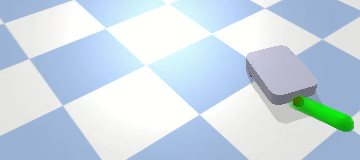
\includegraphics[width=0.95\textwidth]{4_non_holonomic/simBoxer/boxer_dynamic_fabrics_7_cropped.png}
    \caption{7s}
  \end{subfigure}%
  \begin{subfigure}{0.3\linewidth}
    \centering
    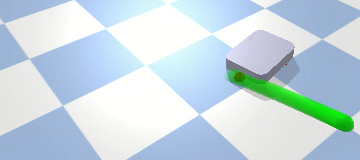
\includegraphics[width=0.95\textwidth]{4_non_holonomic/simBoxer/boxer_dynamic_fabrics_11_cropped.png}
    \caption{11s}
  \end{subfigure}%
  \begin{subfigure}{0.3\linewidth}
    \centering
    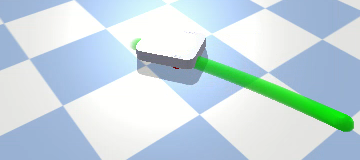
\includegraphics[width=0.95\textwidth]{4_non_holonomic/simBoxer/boxer_dynamic_fabrics_18_cropped.png}
    \caption{18s}
  \end{subfigure}
  \begin{subfigure}{0.3\linewidth}
    \centering
    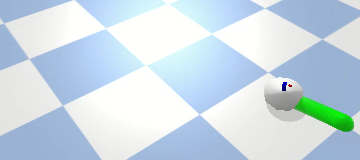
\includegraphics[width=0.95\textwidth]{4_non_holonomic/simBoxer/point_dynamic_fabrics_7_cropped.png}
    \caption{7s}
  \end{subfigure}%
  \begin{subfigure}{0.3\linewidth}
    \centering
    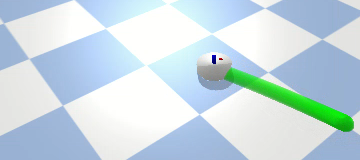
\includegraphics[width=0.95\textwidth]{4_non_holonomic/simBoxer/point_dynamic_fabrics_11_cropped.png}
    \caption{11s}
  \end{subfigure}%
  \begin{subfigure}{0.3\linewidth}
    \centering
    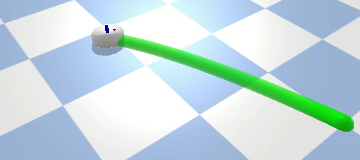
\includegraphics[width=0.95\textwidth]{4_non_holonomic/simBoxer/point_dynamic_fabrics_18_cropped.png}
    \caption{18s}
  \end{subfigure}%
  \caption{Path (green) following with a holonomic and a non\hyp{}holonomic robot using \ac{df} with the extension
  to non\hyp{}holonomic robots}
  \label{fig:non_holonomic_trajectory}
\end{figure}

% \subsection{Limitation of the extension}
% \label{sub:limitation_extension}

The theory of optimization fabrics is built upon energy conservation of artificial energies
that design the motion. \cref{eq:non_holonomic_fabrics} does not solve the
resulting spec exactly, but minimizes the deviation according to the least square objective function.
For many kinematic systems, e.g., differential drive model, bicycle model, the
non\hyp{}holonomic constraint additionally reduces the number of degrees of freedom, 
$\dim{q} < \dim{x}$. As a consequence, the least square solution has a non-zero residuum.
Then, some fundamental properties of optimization fabrics, such as energy
conservation and convergence can no longer be guaranteed. Despite this theoretical
shortcoming, we show that this approach leads to good performance in practical applications. 









